%!TEX root = ../../report.tex
\section{Summary}
In this chapter various methods of including pose estimation noise into an occupancy grid mapping approach has been evaluated. 
The method that was chosen is the reduced ideal model with pose decay because of its ability to avoid overconfidence in observations made under error-prone localization. 
The occupancy probabilities chosen for free is \(0.4\) and \(0.6\) for occupied. The pose estimation noise is incorporated as a weight that reduces the certainty as the estimation variance increases.  

These elements has been inserted in the static mapper block, as seen in figure \ref{fig:static_map_detail}. 
The sensor input and pose estimation is combined and inserted in the static map as determined by the sensor model and noise weight.
Based on the estimated pose and observed LIDAR scans a static occupancy grid map is created with the sensor model. 
At fixed intervals the static map is then provided as a snapshot to the dynamic learner and then cleared. 

\begin{figure}[htbp]
	\centering
	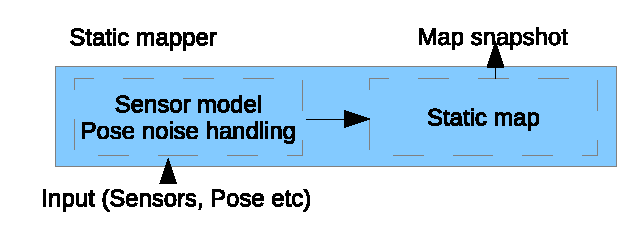
\includegraphics[scale=1]{chapters/static_mapping/figures/static_map_detail.eps}
	\caption{Static mapping module concept}
	\label{fig:static_map_detail}
\end{figure}

